

\section{Observing Klimahusets narrative storytelling in-action}
\par
\emph{Observation and interview 16.02.2022}
\par

After my readings on the museum and its expository agency, I wonder what Klimahuset’s stakeholders thoughts are on their agency? And their position toward whether or not they have a subjective or objective expository agency? What are the cultural attitudes, decisions, views and stances the agents involved in designing the climate exhibition in Klimahuset, took before they decided to do the act of exposing? What cultural function does the objects on display in Klimahuset pose? 

Some of these questions can already kind of be elaborated for, from initial reading on internal documents that I have gotten access through collaborating partners in Klimahuset, as well as from conversations with stakeholders from Klimahuset last semester through the workshop, mail correspondence and mini-exhibition. As accounted for in Klimahusets founding documents, their vision/ purpose of the museum is as follows:
To give the visitors an understanding of the most important climate processes that affect the living conditions on Earth so that they are able to develop their own views on climate change, take part in climate discussions or act in other ways in relation to the topic.
Visitors must gain an understanding that natural conditions also affect social structures and culture.
	
Building on Mieke Bal’s narrative analysis on cultural imperialism in museums, say we look at Klimahuset as an ethnographic museum with the expository agency to display installations, objects and data related to the climate crisis. And with a distinct and clear target group being children aged 10-14. Is Klimahusets agency and vision an attempt to display the climate crisis as a current/ ongoing discourse with the function to educate and stimulate critical reflections on current societal norms and ways of living, or is the agency to define and lay up cultural change, to a more sustainable way of living? Maybe both? If so, then comes the question if the museums cultural stakeholders, with this expository agency, are they cultural moralists? Especially because their whole museum exhibition are designed to engage children aged 10-14, though welcoming all age groups, raises the question if the museum and exhibition design in itself potentially have any moral imperialistic function as well, as to who the discourse (the climate crisis) is relevant for. 
Asked the klimaverter about  this, need to do some structural analysis of some sort….

\begin{figure}[H]
\centering 
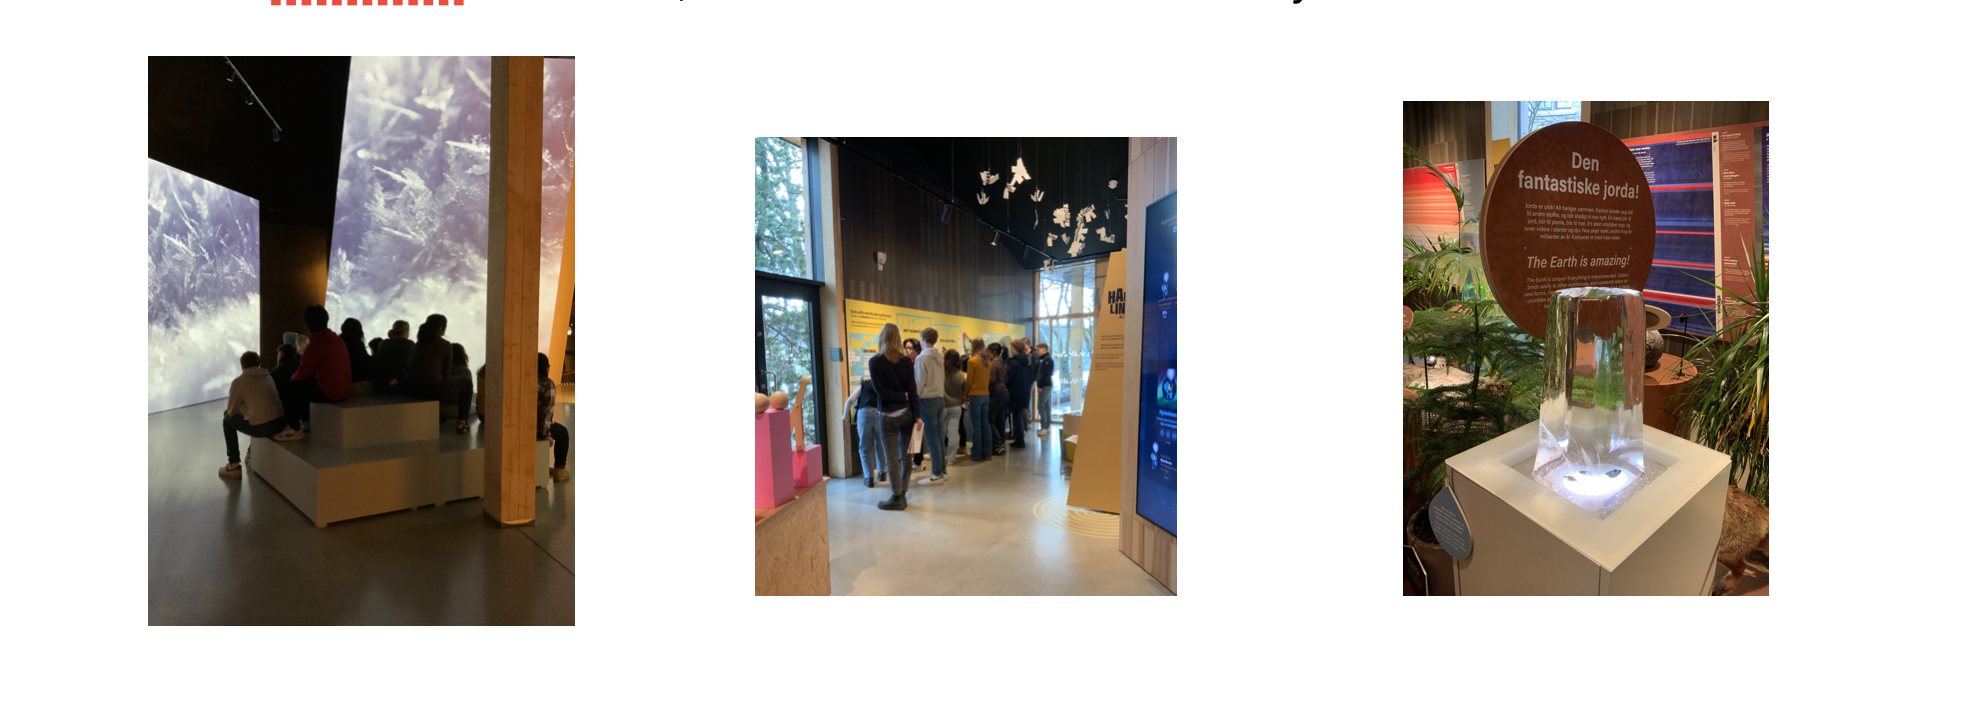
\includegraphics[width=13cm]{pictures/elever_i_klimahuset.png}
\caption{Kids in Klimahuset}
\end{figure}

Med en klimavert til stede får man bedre hjelp og en form for retning til å “lese” installasjonene, som støtter deg når du senere går gjennom avdeling for avdeling. 
% Man blir stilt spørsmål som er knyttet til faktiske ting, som for eksempel i video-atriet sier klimavert; jeg er 160cm høy, hvor høy tror dere denne veggen er?
% Etter litt håndsopprekning får vi vite at dersom Grønlandsisen smelter vil havet stige like høyt som det den veggen er. Det er tankevekkende og setter inntrykk!

Her blir man også litt senere spurt: ser dere vær eller klima? et åpent spørsmål som setter i gang en god diskusjon på forskjellen mellom vær og klima, med fokus på hvordan vær påvirker klima. Dette blir forklart at mange blander og tenker at vær og klima er det samme, og at klimaforandringer og værforandringer ikke er det samme. Her får noen elever aha-øyeblikk.


Et annet eksempel er isbiten inne i “den naturlige avdelingen”.  Først får elevene i oppgave å finne noe i området som påvirker klimaet naturlig. Senere når det blir tatt en liten runde spør verten; har alle tatt på isbiten? For så å gå videre til å forklare hvordan menneskelig påvirkning påvirker klimaet. “For eksempel har deres varme hender bidratt til å smelte litt av isbiten her i Klimahuset”. Dette er også tankevekkende og setter inntrykk!



\section{The role of prototyping in this thesis}
Research through design is a type of research practise where the researcher create artefact- or object prototypes to gain the necessary insight needed to drive and conduct the research project. Prototyping, or the use of prototypes can be used in a variety of ways, and in every stage throughout the project. In the field of human-computer interaction (HCI), software engineering and design, the term prototype is commonly used to signify a specific kind of object used in the design process \autocite[p. 2]{lim_anatomy_2008}. The prototypes are either physical or digital, and function as either a speculative solution, as a manifestation of a design idea, or to explore a design space - all in relation to the research scope and focus. Prototypes are the means by which designers organically and evolutionary learn, discover, generate and refine designs \autocite[p. 2]{lim_anatomy_2008}. They are design-thinking enablers deeply embedded and immersed in design practise, not just as tools for evaluating or proving successes or failures of design outcomes \autocite[p. 2]{lim_anatomy_2008}


In the search for a new way of thinking about prototypes and prototyping, based on the need for exploring and establishing a definition that differs from current approaches in software engineering contexts where engineers use prototypes to identify or satisfy requirements: Lim et. al., conceptualise prototypes as tools for traversing a design space where all possible design alternatives and their rationales can be explored \autocite[p. 2]{lim_anatomy_2008}. In that way, the prototype serves as a communicative manifestation, where the designer is enabled to communicate the rationales of their design decisions through the prototype \autocite[p. 2]{lim_anatomy_2008}. Prototypes stimulate reflections, and designers use them to frame, refine and discover possibilities in a design space \autocite[p. 2]{lim_anatomy_2008}. This new way of thinking about prototypes differs markedly from requirement-oriented approaches like software engineering, recognising design activities as flexible rather than rigid, reflective rather than prescriptive, and problem-setting rather than problem-solving (Schön, 1982). A design idea that satisfies all the identified requirements does not guarantee that it is the best design since a number of ways can meet each requirement \autocite[p. 2]{lim_anatomy_2008}. If the focus of prototyping is framing and exploring a design space, what matters is not identifying or satisfying requirements using prototypes but finding the manifestation that in its simplest form, filters the qualities in which designers are interested, without distorting the understanding of the whole \autocite[p. 2]{lim_anatomy_2008}. In order to support this perspective and to provide a stable foundation for the study of prototypes in HCI, Lim et. al. (2008) proposes a framework for conceptualising prototypes. The framework is an attempt to create an understanding of the nature of prototypes in general and to provide a language for articulating the characteristics of a particular prototype \autocite[p. 3]{lim_anatomy_2008}. Two fundamental aspects of prototyping form the basis of the framework:

1) prototypes are for traversing a design space, leading to the creation of meaningful knowledge about the final design as envisioned in the process of design, and
2) prototypes are purposefully formed manifestations of design ideas.
\autocite[p. 3]{lim_anatomy_2008}

In the reflection process of these questions,
\begin{itemize}
    \item What values are important in my context?
    \item What is my design outcomes?
    \item What is my design space?
    \item Experience prototyping? Am I going to prototype an experience?
    \item Why and how do I intend a particular prototype to support the design process?
\end{itemize}

I decided that it would be for the best in this context to analyse other installations. Experiences from the tangible course, plus time to build vs analyse/ write. 


In my attempt to answer how one can design meaningful interactive experiences in a museum space that addresses sustainability, I have chosen to look into three theoretical frameworks that give the means to understand interactive artefacts dialogic qualities - as an answer to how museum spaces can look at their respective installations and judge whether or not they stimulate the visitor to dialogue (conversations). The hypothesis is that there lies value for the museum to judge whether or not their installations promote dialogue. 


\section{Qualitative research (very unfinished!)}
Flytte til diskusjon? Heller skrive ut om literature review steget?
jeg gjør kritisk forskning: critical design of existing artifacts instead of designing my own. To proper explore Rq I would need t omake a lot of designs, not enough time, better to lean on theory and explore existing installations so that I can actually explore more of them and "talk back to theory". I use theory to analyse installations installations with a design perspective: user experience (meaningful) and dialogical interactive elements/ qualities. 


My knowledge outcomes from this thesis project:
\begin{itemize}
    \item Proposal of a theoretical lens to read and understand a interactive installations in the museum/ an exhibition. To identify meaningful relations between the dissemination and exhibition practise.
    \item A critical view on the topic of interactivity addressing contemporary topics/issues in a museum space
    \item 
\end{itemize}

\section{Interview with a concept developer from Munch}
\par
\emph{date date date}
\par

\emph{"Det beste er jo når folk lærer noe nytt uten at de merker det, det burde jo være målet og det kan jo være tekst for eksempel som byr på en veldig engasjerende historie men det kan også være noe interaktivt, f.eks. du tar en selfie og at Munch også gjorde det og lagde disse effektene, og kanskje man blir litt interessert i det og kan finne ut mer om det andre steder i museet, som f.eks. i “uendelig utstilling” er det også sånn at vi mener at de forskjellige utstillinger er jo ..(?) av hverandre (at de bygger på hverandre?) og skaper altså verdi for hverandre, at folk som har vært i skygger har muligheten å oppleve Munchs kunst på nye måter ved gå inn i uendelige [avdeling]. Men vi jobber også med nye utstillingsprosjekter der vi, der den tilknytningen mellom digitale opplevelser og mer tradisjonelle presentasjoner av kunst er mer tettere, f.eks. at du at man har sånne immersive rom eller opplevelser i en utstillingssal man kan gå inn i og så ut igjen og oppleve kunsten på en ny måte. Det syns vi er en veldig produktiv måte for å åpne opp utstillingssaler for et større publikum og engasjere flere og bredere. [Her sier B: ja flere perspektiver eller, men tok ikke det på egen linje]. Ja. Vi ser det også med Poison [utstilling] f.eks., mange som likte det hadde også behov for å se originalbildene f.eks. Så det tror jeg er absolutt noe som ikke erstatter originalkunsten, som mange frykter, men må være som beriker og gir deg kanskje en, gir også visse grupper en sjans for at de gidder å befatte seg med det eller se på kunsten og ikke bare, de fleste ser jo bare i 3 eller 5 sekunder på et bilde og så gå videre til neste. Uten formiddling er det ikke noen sjanse for å øke den tiden enkelte tilbringer med kunsten."}


\section{from klimahuset observation}
Med en klimavert til stede får man bedre hjelp og en form for retning til å “lese” installasjonene, som støtter deg når du senere går gjennom avdeling for avdeling. 
Man blir stilt spørsmål som er knyttet til faktiske ting, som for eksempel i video-atriet sier klimavert; jeg er 160cm høy, hvor høy tror dere denne veggen er?
Etter litt håndsopprekning får vi vite at dersom Grønlandsisen smelter vil havet stige like høyt som det den veggen er. Det er tankevekkende og setter inntrykk!

Her blir man også litt senere spurt: ser dere vær eller klima? et åpent spørsmål som setter i gang en god diskusjon på forskjellen mellom vær og klima, med fokus på hvordan vær påvirker klima. Dette blir forklart at mange blander og tenker at vær og klima er det samme, og at klimaforandringer og værforandringer ikke er det samme. Her får noen elever aha-øyeblikk.


Et annet eksempel er isbiten inne i “den naturlige avdelingen”.  Først får elevene i oppgave å finne noe i området som påvirker klimaet naturlig. Senere når det blir tatt en liten runde spør verten; har alle tatt på isbiten? For så å gå videre til å forklare hvordan menneskelig påvirkning påvirker klimaet. “For eksempel har deres varme hender bidratt til å smelte litt av isbiten her i Klimahuset”. Dette er også tankevekkende og setter inntrykk!